\documentclass[11pt,a4paper]{article}
\usepackage[margin=2.0cm,top=1.8cm,bottom=1.8cm]{geometry}
\usepackage[T1]{fontenc}
\usepackage[utf8]{inputenc}
\usepackage{lmodern}
\usepackage{amsmath,amssymb}
\usepackage{siunitx}
\usepackage{booktabs}
\usepackage{graphicx}
\usepackage{caption}
\usepackage[hidelinks]{hyperref}
\sisetup{separate-uncertainty=true,per-mode=symbol}
\captionsetup{font=small,labelfont=bf,skip=4pt}
\setlength{\textfloatsep}{8pt}\setlength{\intextsep}{8pt}
\setlength{\parskip}{2pt}

\title{\vspace{-1.3cm}Problem Set 1 --- Equilibrium bond length of H$_2$ with DFT}
\author{Vladimir Jurien}
\date{\today}

\begin{document}
\maketitle
\vspace{-1.1cm}

\section*{Method}
Total energies of H$_2$ were computed with \texttt{pw.x} (Quantum ESPRESSO \cite{QE}) using the
supplied input \texttt{H2.in}. The numerical settings were kept fixed: \SI{12}{\angstrom} cubic
box, \SI{60}{Ry} plane-wave cutoff, $\Gamma$ point only. Only the bond length $b$ ($z$-coordinate
of the second H atom) was varied, from 0.60 to \SI{1.20}{\angstrom} in steps of \SI{0.04}{\angstrom},
and for part~(c) the pseudopotential was changed from \texttt{H.pz-vbc.UPF} (LDA) to
\texttt{H.pbe-vbc.UPF} (GGA--PBE \cite{PBE}). All SCF calculations converged.

\section*{(a) Energy versus bond length}
The LDA total energies are listed in Table~\ref{tab:data} (PBE values from part~(c) alongside)
and plotted in Fig.~\ref{fig:both}(a). The lowest LDA total energy on the grid is at
\[
  b = \SI{0.76}{\angstrom}, \qquad E = \SI{-2.27200515}{Ry}.
\]
(LDA and PBE total energies are each defined only within their own functional and pseudopotential
and are not compared with each other.)

\begin{table}[htb]
\centering
\caption{Total energy of H$_2$ versus bond length from \texttt{pw.x} (\SI{60}{Ry},
\SI{12}{\angstrom} box, $\Gamma$ point). Lowest grid point in bold.}
\label{tab:data}
\footnotesize
\begin{tabular}{S[table-format=1.2] S[table-format=-1.8] S[table-format=-1.8] @{\hspace{1.4cm}} S[table-format=1.2] S[table-format=-1.8] S[table-format=-1.8]}
\toprule
{$b$ (\si{\angstrom})} & {$E_\text{LDA}$ (Ry)} & {$E_\text{PBE}$ (Ry)} & {$b$ (\si{\angstrom})} & {$E_\text{LDA}$ (Ry)} & {$E_\text{PBE}$ (Ry)} \\
\midrule
0.60 & -2.22352148 & -2.28370102 & 0.92 & -2.25120042 & -2.30067764 \\
0.64 & -2.24671146 & -2.30503490 & 0.96 & -2.24128285 & -2.28988421 \\
0.68 & -2.26131788 & -2.31801191 & 1.00 & -2.23030085 & -2.27810958 \\
0.72 & -2.26924915 & -2.32447971 & 1.04 & -2.21851510 & -2.26560794 \\
0.76 & \bfseries -2.27200515 & \bfseries -2.32589317 & 1.08 & -2.20613839 & -2.25258417 \\
0.80 & -2.27075872 & -2.32340442 & 1.12 & -2.19334916 & -2.23920953 \\
0.84 & -2.26642664 & -2.31792429 & 1.16 & -2.18030016 & -2.22563023 \\
0.88 & -2.25972301 & -2.31016518 & 1.20 & -2.16712226 & -2.21197218 \\
\bottomrule
\end{tabular}
\end{table}

\begin{figure}[htb]
\centering
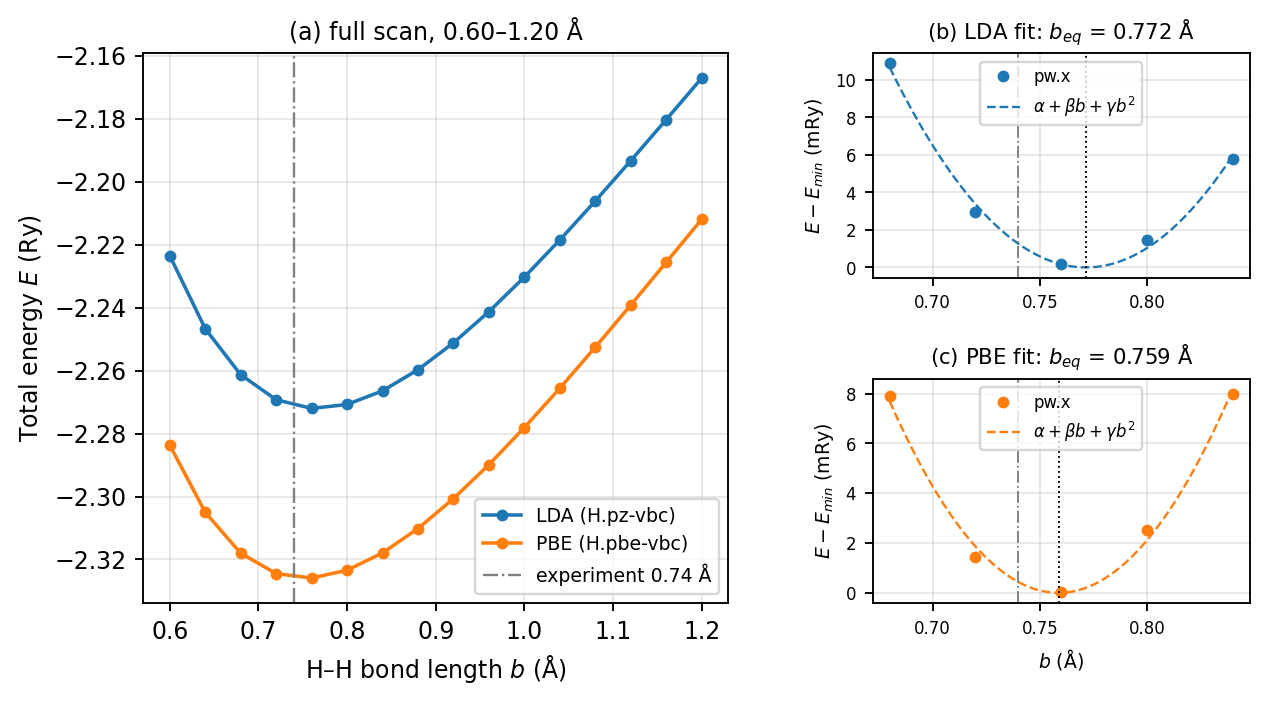
\includegraphics[width=0.9\textwidth]{both_curves.png}
\caption{(a) Total energy of H$_2$ versus bond length for LDA (\texttt{H.pz-vbc}) and PBE
(\texttt{H.pbe-vbc}); the dash-dotted line marks the experimental bond length. (b), (c) The five
points used in the quadratic fit for LDA and PBE, relative to the fitted minimum, with the fitted
parabola (dashed) and $b_\text{eq}$ (dotted).}
\label{fig:both}
\end{figure}

\section*{(b) Quadratic fit}
Near the minimum the curve was fitted with $E(b)=\alpha+\beta b+\gamma b^2$; setting
$\mathrm{d}E/\mathrm{d}b=\beta+2\gamma b=0$ gives $b_\text{eq}=-\beta/(2\gamma)$. The fit used
\texttt{numpy.polyfit(b,E,2)}, which returns the coefficients highest power first,
$[\gamma,\beta,\alpha]$. A parabola is only a valid model close to the minimum (the curve is
steep on the compressed side and flattens towards dissociation), so I used the five points within
$\pm\SI{0.10}{\angstrom}$ of the lowest grid point, $b=0.68$--\SI{0.84}{\angstrom}: the smallest
symmetric window that still over-determines the three parameters. Table~\ref{tab:window} shows that
wider windows pull $b_\text{eq}$ systematically outward; the spread between the 3-, 5- and 7-point
fits, $\pm\SI{0.005}{\angstrom}$, is taken as the uncertainty of $b_\text{eq}$. For LDA:
\[
  \alpha = \SI{-1.514102}{Ry},\quad
  \beta  = \SI{-1.965223}{Ry\per\angstrom},\quad
  \gamma = \SI{1.273622}{Ry\per\angstrom\squared},\qquad
  b_\text{eq}^\text{LDA} = -\frac{\beta}{2\gamma} = \SI{0.772}{\angstrom}.
\]

\begin{table}[htb]
\centering
\caption{Sensitivity of the fitted $b_\text{eq}$ to the fit window (half-width around
$b=\SI{0.76}{\angstrom}$). The window used is in bold.}
\label{tab:window}
\small
\begin{tabular}{S[table-format=1.2] c S[table-format=1.4] S[table-format=1.4]}
\toprule
{half-width (\si{\angstrom})} & points & {$b_\text{eq}^\text{LDA}$ (\si{\angstrom})} & {$b_\text{eq}^\text{PBE}$ (\si{\angstrom})} \\
\midrule
0.06 & 3  & 0.7675 & 0.7545 \\
\bfseries 0.10 & \textbf{5} & \bfseries 0.7715 & \bfseries 0.7587 \\
0.14 & 7  & 0.7773 & 0.7650 \\
0.30 & 12 & 0.7990 & 0.7830 \\
\bottomrule
\end{tabular}
\end{table}

\section*{(c) GGA--PBE and comparison with LDA and experiment}
With \texttt{H.pbe-vbc.UPF} the lowest grid point is again $b=\SI{0.76}{\angstrom}$
($E=\SI{-2.32589317}{Ry}$, Table~\ref{tab:data}, Fig.~\ref{fig:both}). The same five-point fit gives
\[
  \alpha = \SI{-1.611497}{Ry},\quad
  \beta  = \SI{-1.883171}{Ry\per\angstrom},\quad
  \gamma = \SI{1.240985}{Ry\per\angstrom\squared},\qquad
  b_\text{eq}^\text{PBE} = \SI{0.759}{\angstrom}.
\]
A check with a \SI{100}{Ry} cutoff and a \SI{16}{\angstrom} box changed both $b_\text{eq}$ values by
less than \SI{0.001}{\angstrom}.

\begin{table}[htb]
\centering
\caption{Equilibrium bond length of H$_2$ compared with the experimental value
\SI{0.74}{\angstrom}.}
\label{tab:compare}
\small
\begin{tabular}{l l l}
\toprule
Method & $b_\text{eq}$ (\si{\angstrom}) & error vs.\ \SI{0.74}{\angstrom} \\
\midrule
LDA (\texttt{H.pz-vbc.UPF})  & $0.772\pm0.005$ & $+4.3\,\%$ \\
PBE (\texttt{H.pbe-vbc.UPF}) & $0.759\pm0.005$ & $+2.5\,\%$ \\
Experiment                   & $0.74$          & --- \\
\bottomrule
\end{tabular}
\end{table}

Both functionals overestimate the bond length; PBE reduces the error from 4.3\,\% to 2.5\,\%. LDA
evaluates the exchange--correlation energy at each point as if the density there were a uniform
electron gas, which is a poor description of H$_2$, whose density is strongly peaked at the two
nuclei and decays exponentially away from them. PBE adds a dependence on the density gradient
$|\nabla n|$, which describes such inhomogeneous densities better and brings the bond length closer
to experiment. The PBE curvature $\gamma$ is also slightly smaller, i.e.\ the bond is marginally
softer. The remaining error reflects the approximate functional and pseudopotential.

\begin{thebibliography}{9}\footnotesize\setlength{\itemsep}{0pt}
\bibitem{QE} P.~Giannozzi \emph{et al.}, J.\ Phys.: Condens.\ Matter \textbf{21}, 395502 (2009);
  \textbf{29}, 465901 (2017).
\bibitem{PBE} J.~P.~Perdew, K.~Burke and M.~Ernzerhof, Phys.\ Rev.\ Lett.\ \textbf{77}, 3865 (1996).
\end{thebibliography}
\end{document}
